\documentclass[conference]{IEEEtran}
\usepackage[utf8]{inputenc}
\usepackage{ifpdf}
\renewcommand{\sfdefault}{cmss}
\renewcommand{\rmdefault}{cmr}
\renewcommand{\ttdefault}{cmtt}
\usepackage[english,russian]{babel}
\usepackage[pdftex]{graphicx}
\usepackage{listings}
\usepackage{caption}
\usepackage[colorlinks,filecolor=blue,citecolor=green,unicode,pdftex]{hyperref}
\usepackage{cmap}
\hypersetup{colorlinks=true, linkcolor=blue, citecolor=blue, filecolor=blue, urlcolor=blue, pdftitle=1, pdfauthor=, pdfsubject=, pdfkeywords=}

\begin{document}

\title{Тестирование среды программирования роботов}

\author{
	\IEEEauthorblockN{Д.А. Мордвинов}
	\IEEEauthorblockA{
		Санкт-Петербургский государственный университет\\
		Кафедра системного программирования\\
		Email: mordvinov.dmitry@gmail.com
	}
\and
	\IEEEauthorblockN{Ю.В. Литвинов}
	\IEEEauthorblockA{
		Санкт-Петербургский государственный университет\\
		Кафедра системного программирования\\
		Email: y.litvinov@spbu.ru
	}
}

\maketitle

\begin{abstract}
В статье представлен опыт тестирования достаточно сложной визуальной среды программирования роботов, 
написанной на C++ с использованием библиотеки Qt. Рассматриваются три аспекта тестирования среды --- 
модульное тестирование, тестирование пользовательского интерфейса и функциональное тестирование посредством 
интерпретации программ, написанных в среде, на имитационной модели с заданными ограничениями на состояние модели. 
Приводится описание языка задания ограничений. Описываются другие задачи, помимо тестирования, где представленные 
в статье решения оказались полезны --- код для тестирования пользовательского интерфейса переиспользован для 
реализации режима обучения, код для функционального тестирования переиспользован для проверки заданий учащихся 
онлайн-курса. Статья может быть полезна специалистом, занимающимся разработкой приложений на C++ с Qt и людям, 
занимающимся тестированием с использованием имитационных моделей физических объектов, которыми управляет программа.
\end{abstract}

\section{Введение}
C 2012 года ведётся разработка робототехнического конструктора ТРИК\footnote{Домашняя страница конструктора ТРИК, URL: http://www.trikset.com/ (дата обращения: 17.08.2015)} 
и графической среды программирования для него TRIK Studio~\cite{litvinov2015trikstudio}. Среда программирования 
появилась на базе наших исследований в области визуального моделирования (\cite{kuzenkova2013qreal, kuzenkova2011qreal, terekhov2009architecture}) 
и их приложения к робототехнике (\cite{terekhov2013robots, litvinov2012robots, tikhonova2012robots, bryksin2011robots}), 
так что на данный момент она представляет собой достаточно большую и богатую функциональными возможностями 
систему, имеющую несколько тысяч пользователей по всей стране и в мире. Среда предназначается прежде всего 
для обучения школьников и студентов программированию и робототехнике. Система имеет открытый исходный 
код, кроссплатформенная\footnote{Репозиторий проекта на GitHub, URL: http://github.com/qreal/qreal/ (дата обращения: 17.08.2015)} 
(на момент написания статьи работает под управлением операционных систем Windows, Linux и Mac OS X), реализована 
на языке C++ с использованием библиотеки Qt 5\footnote{Домашняя страница библиотеки Qt, URL: http://www.qt.io/ (дата обращения: 17.08.2015)}, 
содержит как развитый пользовательский интерфейс, так и сложную внутреннюю логику работы, включающую в 
себя управление реальными роботами и исполнение программ на имитационной модели. Это создаёт некоторые 
сложности в организации автоматического тестирования системы. В этой статье будет рассказано, как эти 
сложности преодолевались и как вообще было организовано автоматическое тестирование, что может быть полезно 
читателю как с чисто технической точки зрения (тестирование приложений с пользовательским интерфейсом, 
реализованных с использованием библиотеки Qt), так и с научной (тестирование среды программирования роботов 
посредством проверки корректности исполнения программ на имитационной модели).

Среда TRIK Studio представляет собой средство визуального программирования роботов, то есть среду, где 
программы представляются в виде набора графических символов (или блоков), реализующих элементарные команды 
роботу (включить моторы, дождаться срабатывания датчика и т.д.). Блоки соединены стрелками, показывающими 
передачу управления. Такой подход довольно типичен для данной предметной области (ближайшие аналоги TRIK Studio 
--- среды Robolab~\cite{portsmore1999robolab}, NXT-G\footnote{Среда программирования NXT-G, URL: http://www.lego.com/ru-ru/mindstorms/learn-to-program (дата обращения: 07.02.2015)}, 
MRDS\footnote{Microsoft Robotics Developer Studio, домашняя страница, URL: https://msdn.microsoft.com/en-us/library/bb648760.aspx (дата обращения: 07.02.2015)}). 
Одна и та же нарисованная программа может быть исполнена на компьютере с посылкой команд реальному роботу, сгенерирована в программу 
на JavaScript, F\# или C и передана роботу для исполнения в автономном режиме, или исполнена на имитационной 
модели, где симулируется робот и его окружение.

Автоматическое тестирование системы TRIK Studio состоит из трёх частей --- модульного тестирования, тестирования 
пользовательского интерфейса и функционального тестирования посредством имитационной модели. Первые две части 
типичны для практически любых приложений с пользовательским интерфейсом, третья же специфична для предметной 
области робототехники --- среда симулирует поведение реального робота и исполняет тестовые программы на нём, 
контролируя состояние среды симуляции посредством задания ограничений на её состояние, зависящих от времени и происходящих событий.

В статье будет рассказано про каждый из упомянутых выше этапов автоматического тестирования. Каждый этап 
представляет собой применение знаний из весьма обширной области, поэтому мы не ставим себе целью подробно 
рассказать про модульное тестирование или тестирование пользовательского интерфейса вообще (это было бы слишком 
амбициозной задачей, к тому же уже решённой в многочисленных статьях и книгах, например, \cite{banerjee2013graphical, kotlyarov2006testing}). 
Цель данной работы --- представить опыт применения некоторых методик тестирования в реальном промышленном 
активно развивающемся проекте, представить и пояснить принятые нами решения.

\section{Модульное тестирование}
Для C++ существует множество библиотек модульного тестирования и единого стандарта 
не существует. Для выбора конкретной библиотеки мы руководствовались такими критериями, 
как скорость и простота написания теста, умение библиотеки работать с исключениями, 
наличие развитого механизма проверок, наличие поддержки создания mock-объектов. 

Библиотека Qt, на основе которой разрабатывается TRIK Studio, имеет в своём составе 
библиотеку модульного тестирования Qt Test, но, несмотря на хорошую интеграцию с Qt, 
нам она не подошла по причине отсутствия встроенной поддержки работы с исключениями 
и mock-объектами. Также были рассмотрены библиотеки CPPUnit, Boost.Test, CppUnitLite, 
Unit++, CxxTest, Google C++ Testing Framework, подробное сравнение этих библиотек можно 
найти в []. В результате была выбрана библиотека Google C++ Testing Framework и её 
расширение для написания mock-объектов Google C++ Mocking Framework. Эти инструменты 
удовлетворяют нашим критериям, кроме того, оказались просты в использовании, в том 
числе и в кроссплатформенном окружении. 

Тестовое покрытие TRIK Studio по историческим причинам неравномерно. Наиболее полно 
покрыта тестами функциональность, реализованная в течение последних двух лет (в то время, 
когда проект вырос из студенческого проекта в промышленную разработку), кроме того, 
преимущество отдавалось функциональности, хорошо подходящей для модульного тестирования 
--- например, синтаксический анализатор и интерпретатор встроенного в TRIK Studio 
текстового языка, а также средство проверки корректности работы программ (о котором ниже) 
покрыты тестами наиболее полно. При написании тестов мы пытались поддерживать соответствие 
"`один исполняемый файл с тестами --- один бинарный файл системы (разделяемая библиотека 
или исполнимый файл)"', структура тестов примерно повторяет структуру основного проекта. 
При этом возникла проблема, что операционная система Windows не позволяет передавать 
в командной строке слишком длинные пути (более примерно 250 символов), поэтому пришлось 
несколько упростить в тестах иерархию каталогов, иначе возникали трудности со сборкой. 
Модульные тесты не раз доказали свою эффективность, помогая искать ошибки на ранних этапах 
разработки и упрощая рефакторинг.

\section{Тестирование пользовательского интерфейса}
Одно лишь модульное тестирование, по крайней мере в нашем случае, не может покрыть 
все аспекты системы. Пользовательский интерфейс также подлежит проверке корректности. 
Данный раздел содержит описание результатов поиска подходящего решения, подхода к 
тестированию пользовательского интерфейса в TRIK Studio, а также обсуждение некоторых 
прикладных сторон технологии, полученной в результате данного исследования.

\subsection{Существующие подходы}
Тестирование графических интерфейсов --- область, возраст которой составляет четверть 
века. За это время были опубликованы сотни статей, проведена их подробная классификация 
(ссылка на http://www.cs.umd.edu/~baonn/papers/ist2013.pdf), разработано большое количество 
подходов и инструментов, реализующих эти подходы. Наша работа не затрагивает фундаментальных 
теоретических оснований данной области, а скорее является ценным практическим результатом 
на пересечении технологий, о которых будет рассказано в этом и последующих разделах.

Мы имеем дело со сложным и постоянно совершенствующимся интерфейсом, созданным на 
основе инструментария Qt Widgets. Кроссплатформенность системы предъявляет важное 
требование к технологии тестирования интерфейса --- одни и те же тесты должны иметь 
работать на различных операционных системах, оконных менеджерах, установленных разрешениях 
экрана и т.д. Открытость кода и свободное распространение среды делает непригодными 
коммерческие системы тестирования (например, Squish, который пригоден по всем другим 
параметрам). Приведем обзор технологий, с которыми мы столкнулись в процессе поиска 
конечного решения задачи тестирования интерфейсов.

\subsubsection{Библиотека Qt Test}
Инструментарий Qt содержит набор средств автоматизации взаимодействия с пользовательским 
интерфейсом приложения, предоставляя библиотеку Qt Test в базовом некоммерческом модуле. 
Данный инструмент позволяет автоматизировать взаимодействие с графическим интерфейсом 
посредством задержек и эмулирования низкоуровневых событий мыши и клавиатуры. Высокоуровневые 
операции поиска и взаимодействия с определенными элементами управления, инструменты 
их поиска и определения отсутствуют в библиотеке Qt Test, тем не менее содержатся 
в том или ином виде в различных местах инструментария для создания самих интерфейсов. 

В результате тест с использованием данной библиотеки представляет собой модуль на 
C++, требующий самостоятельной реализации частых операций (например, создание операции 
drag-and-drop из одного места в другое с последующим использованием результатов этой 
операции), а также перекомпиляции тестов при изменении пользовательского интерфейса, 
что затрудняет их поддержку. Сами по себе эти факторы не кажутся чрезмерно проблематичными, 
однако на практике показали себя довольно затрудняющими процесс создания и поддержки 
тестов, код получался громоздким, появилось понимание, что создание тестов на скриптовом 
языке подошло бы гораздо лучше.

Тем не менее, формально данная технология удовлетворяет всем нашим требованиям, тесты 
не зависят от платформы, изменение интерфейса требует сопоставимых изменений тестов.

\subsubsection{Windows Automation API}
Для тестирования пользовательского интерфейса Windows-приложений часто используются 
возможности операционной системы Windows, а именно Windows Automation API. Это набор 
функций, доступных как из .NET, так и для программ на C++, с помощью которых можно 
получить доступ к элементам пользовательского интерфейса, таким как кнопки, поля для 
ввода, списки и т.д., и симулировать события ввода. В составе Windows SDK поставляются 
программы Inspect и AccScope, использующие Automation API для того, чтобы показывать 
структуру и свойства элементов управления приложений. Существуют и полноценные библиотеки 
GUI-тестирования, такие как White или UI Automation Verify, скрывающие от программиста 
сложность использования Automation API и позволяющие удобно писать тестовые сценарии на 
.NET, работая в терминах элементов пользовательского интерфейса.

Основной недостаток подобного подхода для нас --- отсутствие кроссплатформенности 
и некоторая ориентированность на .NET (сам Automation API может использоваться и из 
кода на C++, но большинство библиотек к нему написаны на C\#), что хоть и не делает 
невозможным, но усложняет использование такого подхода.

\subsubsection{Sikuli}
Sikuli --- это свободный инструмент, разрабатываемый в MIT для скриптования пользовательских 
действий на основе изображений отдельных областей экрана. Тест представляет собой 
скрипт на языке Python, где в качестве примитива может быть использовано изображение 
какого-либо фрагмента экрана. Инструмент предоставляет удобную среду программирования 
таких скриптов Sikuli IDE, которая удобно отображает и позволяет быстро создавать 
и менять изображения прямо в коде теста.

Удобство написания простых тестов намного выше, чем при использовании библиотеки Qt Test, 
а также исчезают такие проблемы, как манипулирование системными диалогами, однако 
данный инструмент не подошел нам из-за требований кроссплатформенности тестов. Очевидно, 
что на различных платформах и даже в разных версиях одной и той же платформы интерфейс 
приложения может выглядеть совершенно по-разному. При незначительной модификации интерфейса 
зачастую приходилось полностью изменять содержимое тестов. В итоге, несмотря на удобство 
и легкость написания простых тестов, данное обстоятельство делает Sikuli непригодным в нашем случае.

\subsection{Скриптовый программный интерфейс}
В результате так и не было найдено готового решения, способного удовлетворить всем 
поставленным ограничениям. Наиболее близкой к желаемому оказалась библиотека Qt Test, 
которая представляет собой скорее основу для технологии тестирования интерфейсов, чем 
саму технологию. Опыт использования описанных решений позволил нам сформировать представление 
о платформе, обладающей всеми достоинствами Qt Test в виде кроссплатформенности и 
возможности создания самой изощренной логики тестирования и простотой и лаконичностью 
скриптового подхода наподобие Sikuli.

В нашем представлении подходу с использованием Qt Test не хватает "`скриптовости"' и 
высокоуровневости в смысле работы в терминах элементов управления, а не событий от 
манипуляторов. Эти идеи были учтены при реализации системы тестирования интерфейсов TRIK Studio.

В качестве основного языка написания тестов был выбран Qt Script. Это реализация стандарта 
ECMA Script (наиболее популярной реализацией которого является язык JavaScript), расширенная 
механизмами интеграции с Qt-приложениями. Скриптовое окружение расширено инструментами 
работы с пользовательским интерфейсом системы в терминах самого интерфейса. Работа 
этого окружения осуществляется посредством библиотек Qt Test и Qt Widgets, таким образом, 
сохраняются независимость тестов от платформы и легкость доступа ко всем элементам 
управления, при этом решаются проблемы громоздкости кода тестов и низкоуровневости 
терминов, в которых они работают.

Окружение предоставляет доступ ко всем частям интерфейса и методам работы с ними и 
содержит множество методик, специфичных только для TRIK Studio. К примеру, существует 
возможность скриптования создания визуальных диаграмм, рисования модели мира, в котором 
будет производиться имитационное моделирование робота, работы с жестами мышью, изменения 
свойств примитивов, из которых строится программа, работы с настройками приложения, 
управления состоянием вспомогательных панелей и т.д. Реализованы также методы произвольного 
доступа к элементам управления интерфейса по структурному описанию (идентификаторам 
и/или положению в дереве элементов управления) и координатам на экране. Управление 
эмуляторами устройств ввода (например, навигация и действия виртуальной мышью или 
указание клавиатурного фокуса и последовательностей нажатий на кнопки клавиатуры) тесно 
интегрировано с различными видами элементов управления. Например, присутствуют отдельные 
функции прокрутки и работы с выпадающими списками. При этом остаются доступными методы 
синтезирования низкоуровневых событий манипуляторов. 

Кроме всего описанного, скриптовый интерфейс системы содержит методы показа информационных 
сообщений, подсвечивания отдельных элементов управления и рисования стрелок-указателей 
на них, анимации виртуального курсора мыши и тому подобных "`показательных"' функций, 
надобность которых будет обсуждаться в разделе 2.4

Тем не менее, остаются открытыми некоторые проблемы, каждая из которых носит чисто 
технический характер. Одна из них --- управление системными диалоговыми окнами. Дело в том, 
что на каждой платформе системные диалоговые окна (такие как диалоги выбора файлов, 
печати, выбора цвета и т.д.) свои и не поддаются контролю системы синтезирования событий, 
используемой в библиотеке Qt Test. Сейчас эта проблема обходится работой с этими диалогами 
как с "`черными ящиками"' --- тесты задают для себя результаты выбора сущностей, редактируемых 
этими диалогами, не прибегая к работе с ними, "`обходя"', таким образом, их на уровень выше. 
Другая проблема --- отсутствие в Qt Test возможности эмулирования ввода с клавиатуры 
на разных языках, что делает невозможной полноценное тестирование локализации среды. 
Все эти проблемы являются, скорее, проблемами библиотеки Qt Test, в то время как с 
нашей стороны единственной на данный момент проблемой является стоимость поддержки 
кодовой базы, что, безусловно, являясь значимым, не будет обсуждаться в рамках этой статьи.

Полученная технология оказалась практически полностью удовлетворяющей нашим потребностям 
в удобстве написания тестов и их переносимости. Важно, что разработкой автоматизированного 
тестирования интерфейса смогли заниматься люди, практически не имеющие прямого отношения 
к разработке и поддержке самой системы и не имеющие опыта программирования на C++.

\subsection{Инфраструктура}
В данном разделе будет кратко описана структура технологии тестирования, описанной 
в разделе 2.2. Общая архитектура всего комплекса представлена на рисунке~\ref{image:architecture}. Основная 
идея состоит в создании новой "`прослойки"' системы, стоящей над всей технологией, 
интерфейса программирования поведения UI. Этот уровень не модифицирует кодовую базу 
системы, тем не менее агрегируя в себе все ее отдельные компоненты. Очевидно, такое 
возможно только в случае развитой и модульной архитектуры тестируемой системы. Здесь 
реализуются все операции, специфичные для только для данной платформы в удобном для 
использования в скриптах виде, а также происходит "`оборачивание"' операций библиотеки Qt Test. 
Интерпретатор Qt Script, занимающийся исполнением кода самих тестов, штатными средствами 
подхватывает окружение, предоставляемое данной компонентой. Очевидно, что необходимости в 
Qt Script в такой архитектуре нет, можно создавать тесты и на компилируемых языках, 
компонуясь с интерфейсом программирования, в этом случае такой новый уровень можно 
рассматривать просто как инструмент повторного использования кода в тестах.

\begin{figure}[!t]
	\centering
	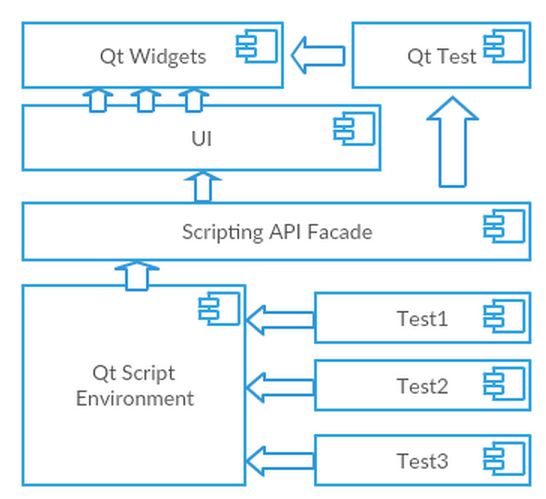
\includegraphics[width=2.5in]{guiTestingArchitecture.png}
	\caption{Архитектура системы тестирования интерфейсов TRIK Studio.}
	\label{image:architecture}
\end{figure}

\subsection{Использование технологии для обучения пользователей}
Полученная технология обладает одним интересным приложением. На базе одной и той же 
инфраструктуры могут быть получены как тесты пользовательского интерфейса, так и автоматизированные 
демонстрации процесса работы со средой, встроенные прямо в нее. Это способ обучения 
пользователя возможностям среды, используемый, в основном, в компьютерных играх --- про 
возможности продукта рассказывает сам продукт (в противоположность, например, таким 
подходам как текстовая справка или видео уроки).

Возможно, такой подход будет полезен разработчикам приложений с развитым, нестандартным 
графическим интерфейсом. Написанием скриптов тестирования и скриптов демонстрации 
могут заниматься одни и те же люди, даже не участвующие в написании кода самого приложения. 
Мы в нашем проекте пошли еще дальше.

На данный момент образование --- основная сфера применения TRIK Studio. Поэтому значительную 
долю пользователей составляют преподаватели в школах, учреждениях дополнительного образования, 
на мастер-классах и т.д. Появилась небезосновательная идея, что преподавателям зачастую 
было бы полезно самостоятельно автоматизировать объяснение рутинного материала посредством 
создания демонстраций на основе описываемой в последних разделах технологии. Очевидно 
также, что осваивать скриптовый язык и объемный API среды подавляющее большинство пользователей 
не станут. Поэтому в рамках эксперимента был создан визуальный язык, похожий на визуальный язык 
TRIK Studio, позволяющий легко и быстро создавать демонстрации. Диаграмма на таком 
языке генерируется в код на текстовом языке описания тестов (Qt Script). Более того, 
была реализована генерация кода по записи действий пользователя. Блоки воспроизведения 
таких действий встроены в визуальный язык как один из его элементов.

\subsection{Обсуждение}
В результате получилась технология, позволяющая создавать тесты графического интерфейса 
и встроенные демонстрации возможностей среды в прямом смысле мышью. Тестировщик или 
преподаватель имеет возможность просто производить какие-либо действия с интерфейсом 
среды, а сама среда затем преобразует эти действия в читаемый код, который может быть 
впоследствии  доработан. Если же требуется реализовать более нелинейную логику работы, 
то имеется возможность создания логики тестирования или демонстрации на визуальном 
языке, с важным подмножеством которого все пользователи уже хорошо знакомы.

Все описанные в разделе 2.4 технологии (визуальный язык, генератор кода теста по действиям 
пользователя, набор встроенных демонстраций) на момент написания статьи проходят апробацию 
и недоступны в официальных версиях. Остальные описанные решения интегрированы в мастер-ветку 
проекта и активно эксплуатируются участниками проекта.

Читателям вряд ли будет полезна идея создания визуального языка описания тестов из-за 
трудоемкости такой работы. В нашем случае мы уже имели готовую технологию быстрого 
создания визуальных предметно-ориентированных языков и генераторов в произвольные языки. 
Идея записи пользовательских действий с последующей генерацией теста уже находила 
свою реализацию, например, в проекте TPTP тестирования приложений, созданных в среде 
разработке Eclipse. Более того, существуют работы, в которых эта методика расширяется 
добавлением элементов искусственного интеллекта [ссылки!].

Однако {ТУТ СКАЗАТЬ, ЗАЧЕМ МЫ ЭТО ПИШЕМ, типа qt, туда сюда, ничего нет, да еще и такой проект}

\section{Функциональное тестирование}
\subsection{Краткое описание возможностей среды}
Далее в этом разделе пойдёт речь о тестировании функциональности, специфичной для 
TRIK Studio (и аналогичных систем, предназначенных для управления некоторым объектом), 
поэтому следует описать подробнее функциональность, которую требуется тестировать. 

Среда TRIK Studio (тогда ещё QReal:Robots) появилась после того, как кибернетики узнали 
о существовании проекта QReal, позволяющего быстро создавать визуальные языки и инструментальные 
средства к ним, и предложили разработать средство программирования для роботов Lego Mindstorms NXT 2.0. 
В результате был разработан прототип, позволявший управлять роботом Lego по интерфейсу 
Bluetooth, интерпретируя диаграмму на компьютере и посылая роботу команды. В дальнейшем 
была добавлена имитационная модель, которая моделировала поведение типового робота --- 
трёхколёсной тележки, режим генерации, позволявший сгенерировать код на C, скомпилировать 
и загрузить на робот для автономного исполнения, а после того, как была добавлена 
поддержка роботов ТРИК, среда была переименована в TRIK Studio, впоследствие была добавлена 
также поддержка конструктора Lego EV3. Общий вид интерфейса среды представлен на рисунке~\ref{image:trikStudio}

\begin{figure*}[!t]
	\centering
	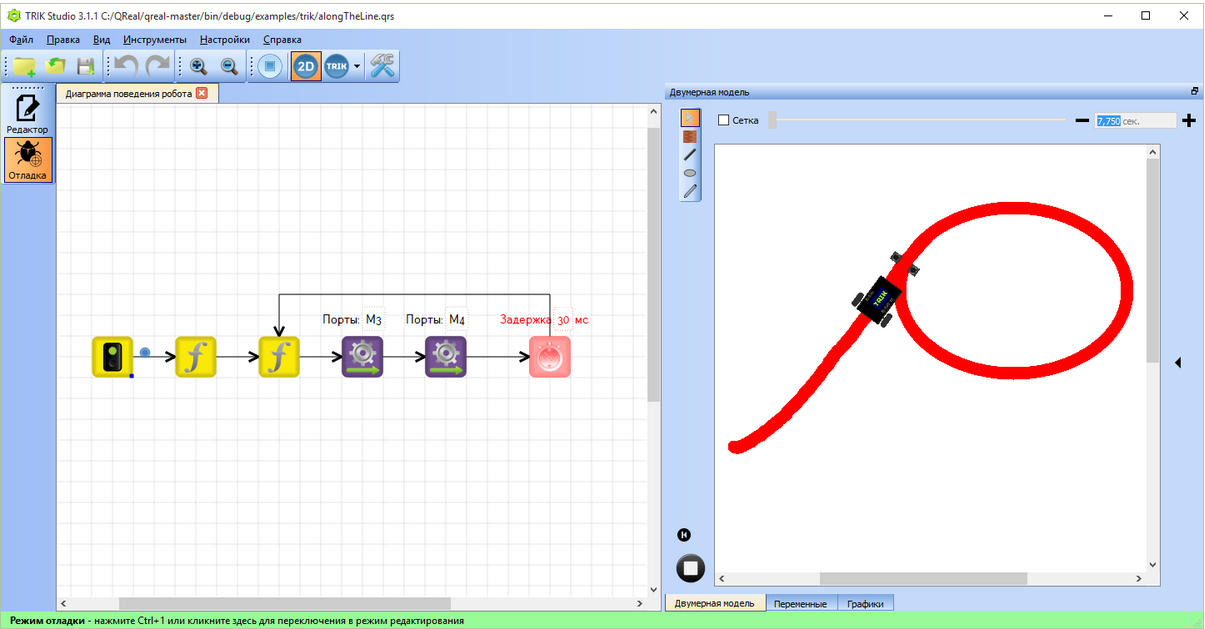
\includegraphics[width=7in]{trikStudio.png}
	\caption{Интерфейс TRIK Studio.}
	\label{image:trikStudio}
\end{figure*}


Программа представляется в виде набора блоков, каждый из которых представляет собой 
элементарную команду роботу или элементарный шаг вычисления. Команды роботу могут 
быть как простыми (например, включить мотор на таком-то порту с такой-то мощностью), 
так и довольно сложными (например, получить данные датчика линии, использующего видеокамеру 
и алгоритмы распознавания изображений), сложные алгоритмы, как правило, реализуются 
на самом роботе и среда лишь вызывает их и обрабатывает результаты. Во всех блоках 
можно использовать математические выражения на текстовом языке, представляющем собой 
подмножество языка Lua 5.3, синтаксический анализатор и интерпретатор которого были 
специально реализованы в TRIK Studio (готовые решения нас не устраивали тем, что невозможно 
было использовать их абстрактное синтаксическое дерево для генерации кода на других 
языках программирования, кроме того, над Lua пришлось реализовать свою систему типов, 
потому что некоторые целевые языки генерации, такие как C, статически типизированы). 
В выражениях можно использовать текущие значения датчиков робота, доступные как специальные 
переменные, они же отображаются в виде таблицы или графиков при запущенной в режиме 
интерпретации программе. В режиме генерации и автономного исполнения обращения к 
таким переменным транслируются в команды чтения значений датчиков и их показания на 
компьютере не отображаются (чтобы дать возможность программе исполняться автономно).

Двумерная модель позволяет исполнять большую часть программ, которые могут быть исполнены 
на реальном роботе. Пользователь может нарисовать в области редактирования двумерной 
модели стены, цветные линии или области на полу, разместить самого робота и его датчики, 
задать им направление. Датчики будут взаимодействовать со стенами и цветными линиями 
(для ТРИК поддержаны инфракрасные и ультразвуковые датчики расстояния, датчик освещённости 
и детектор линии по видеокамере, для Lego NXT или Lego EV3 --- все датчики, входящие 
в стандартный набор: касания, света, цвета и ультразвуковой датчик расстояния). Часть 
функциональности, доступная только на реальном роботе, имитационной моделью не поддерживается, 
например, на данный момент на имитационной модели может быть только один робот, поэтому 
функциональность общения между роботами поддерживать нет смысла. Тем не менее, имитационная 
модель позволяет решать большинство задач из курсов по робототехнике для Lego NXT (например, 
ссылка на книжку Филиппова) и ТРИК (например, ссылка на презентации Ильи), и существенно 
упрощает отладку, давая возможность отладить алгоритм без реального робота, а потом 
лишь подобрать коэффициенты для исполнения той же программы в реальном мире.

Отдельно стоит отметить наличие достаточно развитых средств обеспечения удобства пользовательского 
интерфейса, что связано с образовательной направленностью среды. Например, при рисовании 
диаграмм можно пользоваться механизмом распознавания жестов мышью --- с зажатой правой 
кнопкой рисуется схематичная фигура, которая распознаётся средой и на месте нарисованной 
фигуры создаётся соответствующий ей блок, что позволяет не искать нужный блок в палитре 
и сделать использование среды интереснее для детей. Для TRIK Studio проводились исследования 
по юзабилити и вносились правки в интерфейс по их результатам (см. ссылки на работы Соковиковой и Анастасии Сергеевны).

Генерация кода для автономного исполнения на данный момент реализована для Lego NXT 
в язык C (с использованием библиотеки ECRobot и ОСРВ nxtOSEK) и для ТРИК в языки JavaScript и F\# 
(ссылка на доклады на SECR про этот буллщит). Для ТРИК также реализованы библиотеки 
поддержки времени выполнения на C++ и F\#, которые работают непосредственно на роботе 
и, собственно, реализуют функции, вызываемые программами, сгенерированными в TRIK Studio.

\subsection{Общая схема функционального тестирования}
Поскольку имитационная модель покрывает достаточно большой процент функциональности 
среды и ввиду сложности использования реального робота в автоматических тестах, именно 
имитационная модель используется нами для функционального тестирования. Обычно в аналогичных 
ситуациях пишется эмулятор реального устройства, у нас же эмулятор фактически является 
неотъемлемой частью системы и активно используется конечными пользователями. Предлагаемый 
подход к функциональному тестированию TRIK Studio таков:
\begin{enumerate}
	\item На визуальном языке рисуется программа для исполнения на имитационной модели, 
			решающая ту или иную практическую задачу, а так же рисуется модель мира для 
			имитационной модели, с которым эта программа будет работать.
	\item Программа снабжается описанием ограничений на состояние системы на специальном 
			XML-языке, описание которого приводится ниже. Наборов ограничений для одной 
			программы может быть несколько, при этом они могут использовать разные модели мира.
	\item Файл с сохранённой программой запускается на интерпретацию в двумерной модели, 
			для этого используется специально созданный для нужд тестирования исполняемый 
			файл, представляющий собой по сути TRIK Studio без пользовательского интерфейса. 
			Тестирующая программа перед запуском тестируемой программы подменяет модель мира 
			и набор ограничений в сохранении, что даёт возможность использовать несколько 
			тестов для одной программы. Программа исполняется так, как она исполнялась бы, 
			будучи запущенной пользователем в TRIK Studio, и в случае, если одно из ограничений 
			не выполнено, программа работает некорректно --- делается вывод, что поведение 
			интерпретатора или среды имитационного моделирования отличается от эталонного, 
			тест не пройден.
	\item Тестирующая программа вызывается системой непрерывной интеграции Travis каждый 
			раз после сборки проекта, для всех файлов сохранений и моделей мира для них, 
			имеющихся в репозитории.
	\item Результаты тестов рассылаются по электронной почте разработчикам.
\end{enumerate}

\subsection{Описание языка задания ограничений}
Описание ограничений на имитационную модель робота производится на событийном языке, 
основанном на XML, разработанном как дополнение к механизму имитационного моделирования 
в среде. Выбор в пользу XML-фронтэнда был произведен из чисто практических соображений 
удобства интеграции с описанием остальной имитационной модели мира робота.

Программа на таком языке представляет собой множество { e1, e2, ..., en } событий, где 
каждое событие ei --- это тройка (idi, ci, Ti).

idi --- идентификатор события, внутренняя метка, по которой к событию ei смогут обращаться другие события.
ci --- условие срабатывания события, формула логики первого порядка, о предикатных и функциональных символах которой будет рассказано чуть ниже.
Ti --- упорядоченный список элементарных триггеров [ ti1, ti2, …, tin ]. Элементарный триггер --- это некоторое действие, выполняемое в момент истинности условия срабатывания события ci.

Одному событию соответствует один элемент в XML-спецификации программы. Каждое событие 
в текстовом описании программы может быть представлено либо в виде ограничения, либо в каноническом виде.

Событие в канонической форме --- уже описанная тройка (idi, ci, Ti).

Событие в форме ограничения --- это событие вида (idi, !ci, [ fail(messagej) ]), где “!” означает логическое отрицание, а fail(messagej) --- триггер прекращения исполнения имитационной модели с выдачей сообщения об ошибке messagej. Другими словами, ограничение --- это событие, которое срабатывает тогда, когда нарушается какое-то условие, и которое сообщает об этом нарушении. Особый случай такого ограничения --- лимит времени на выполнение программы. Такое ограничение должно присутствовать в любой программе проверки ограничений имитационной модели TRIK Studio (что проверяется на уровне самого языка задания ограничений), так как проверка, очевидно, не может осуществляться бесконечное время. 

Хоть в выделении ограничений в отдельную группу событий особой надобности нет, на практике удобно описывать утверждения вида ”робот x не должен выезжать за пределы зоны z” или “к роботу x должен быть подключен набор датчиков s” именно в терминах ограничений, а не событий.

Коротко опишем множество доступных в языке предикатных и функциональных символов и элементарных триггеров. Предикатные символы можно поделить на несколько групп:

Предикаты сравнения значений функциональных символов >, <, <=, >=, =, !=.

Пространственные предикаты. Имеют вид “тело x находится внутри области y”.

Предикаты состояния событий settedUp(idi) и dropped(idi), описывающие состояние события (взведено/опущено). Во взведенном состоянии событие может быть выполнено, в опущенном оно остается неактивным, не выполняя триггеры даже при выполнении условия срабатывания события.

Предикат временной прямой timer(t), истинный в моменты модельного времени t и позже.

Прочие предикаты, являющиеся надстройками над уже описанными и поддержанные в целях удобства.

Функциональные символы бывают следующих видов:

Константы различных типов (целочисленные, с плавающей точкой, строковые, логические, цветовые, геометрические и пр.).

Символ variableValue(id) для получения значения переменной с идентификатором id. Переменные могут быть полезны при сложной логике проверки, например, при подсчете числа проделанных роботом итераций.

Арифметические и геометрические операции над значениями других символов, например, модуль числа, подсчет расстояния между двумя точками или выпуклая оболочка множества точек.

Символы сравнения формы двух объектов с использованием расстояния Левенштейна, полезные при проверке схожести фигур, нарисованных роботом.

Символ objectState(path) --- основное средство получения информации о состоянии устройств робота и свойствах предмета из внешнего мира. Аргумент path --- путь к желаемому свойству в иерархии объектов в модели мира. Подробный рассказ обо всех свойствах, предоставляемых окружением, довольно громоздкий и выходит за рамки данной статьи.

Наконец, элементарные триггеры делятся на следующие категории:

success, fail(message) --- управление состоянием проверки. Первый помечает результат проверки как успешный, второй --- как неудавшийся, отображая заданное сообщение об ошибке.

Триггеры задания значения переменных и изменения значения свойств объектов из имитационной модели мира.

Триггеры управления состоянием событий. Каждое событие может взвести или опустить другое или себя, с помощью этого механизма можно задавать сложную логику проверки.

Пример простейшей программы на языке задания ограничений имитационной модели мира в TRIK Studio приведён в листинге~\ref{code:constraints}.

\captionsetup[figure]{name=Листинг}
\setcounter{figure}{0}

\begin{figure*}[!t]
\begin{verbatim}
<!-- Корневой элемент, означающий начало программы проверки ограничений -->
<constraints>

    <!-- Обязательное в любой программе ограничение на время работы -->
    <timelimit value="2000"/>

    <!-- Ограничение на местоположение робота -->
    <constraint failMessage="Робот покинул допустимую зону!">
        <inside objectId="robot1" regionId="warzone"/>
    </constraint>

    <!-- Условие успешности программы: робот должен сказать "Привет" с помощью
        встроенного механизма синтезирования речи и нарисовать улыбку на дисплее -->
    <event settedUpInitially="true">
        <conditions glue="and">
            <equals>
                <objectState object="robot1.shell.lastPhrase"/>
                <string value="Привет"/>
            </equals>
            <equals>
                <objectState object="robot1.display.smiles"/>
                <bool value="true"/>
            </equals>
        </conditions>
        <trigger>
            <success/>
        </trigger>
    </event>

</constraints>
\end{verbatim}
	\caption{Пример программы проверки ограничений имитационной модели мира в TRIK Studio.}
	\label{code:constraints}
\end{figure*}

\subsection{Использование для проверки заданий в онлайн-курсе}
Та же система, что используется для тестирования среды, используется и для проверки 
заданий, сдаваемых пользователями в рамках онлайн-курса по робототехнике, подготавливаемого 
в данный момент для платформы Stepic. На сервере размещён набор задач в виде файлов 
сохранения TRIK Studio, в которых готова (и закрыта для модификации) модель мира для 
имитационной модели, некий набор ограничений, но не до конца нарисована программа 
(или отсутствует вовсе). Учащимся предлагается скачать файл с сохранением, открыть 
его в TRIK Studio, дорисовать программу, проверить, что программа работает у них в 
имитационной модели и удовлетворяет ограничениям, записанным в файле сохранения, и 
загрузить программу на сервер.

На сервере используется та же программа тестирования, которая подменяет модель мира 
и набор ограничений на тестовые и запускает на исполнение пользовательскую программу. 
Возможность подменить модель мира позволяет проверить программу на работоспособность 
в различных (возможно, не известных пользователю заранее) условиях, а различные ограничения 
позволяют управлять случайными факторами, влияющими на работу программы (например, 
датчиком случайных чисел, или симулировать ввод пользователя). По результатам пользователю 
отправляется сообщение с результатом проверки.

Результат работы программы может быть отображён в браузере пользователя с помощью 
JavaScript-программы, рисующей двумерную модель и поведение робота в ходе выполнения 
задачи. Для этого сервер также готовит и отправляет по запросу файл с трассой робота 
--- набором пройденных им точек и состоянием подключенных к нему устройств. Некоторые 
задачи могут быть решены прямо в браузере, без открытия сохранения в TRIK Studio, для 
этого используется среда программирования, частично реализующая возможности TRIK Studio 
на JavaScript. Среда позволяет нарисовать диаграмму, после чего формирует файл сохранения 
TRIK Studio, который открывается как обычно системой проверки.

\subsection{Обсуждение}
Опытный читатель мог заметить, что практически полное подмножество языка задания ограничений 
на поведение роботов в имитационной модели TRIK Studio (все элементы языка, кроме 
конструкций манипулирования состоянием устройств роботов и изменения значения переменных 
и, возможно, некоторые пространственные ограничения и ограничения на состояния объектов, 
которые скорее вспомогательные практические особенности языка, чем существенные его 
элементы) хорошо выражается в терминах темпоральной логики. Действительно, утверждения 
о состоянии устройств робота и событиях представляют собой элементарные предикаты, 
связанные в программе описания ограничений отношениями пропозициональной логики и временными 
отношениями. Общая структура автомата Бюхи, соответствующего формуле темпоральной логики, 
построенной для программы проверки ограничений, будет, скорее всего, напоминать структуру 
автомата, построенного на событиях программы проверки ограничений с их связями. В то же 
время, программа, которую пользователь исполняет в имитационной среде, представляет 
собой визуальную диаграмму, состоящую из набора блоков, связанных стрелками, со множеством 
установленных пользователем свойств, многие из которых легко представимы в виде предикатов 
из предметной области. Очевидно, что описание такой программы легко преобразовать в модель 
Крипке. Все это говорит о том, что, скорее всего, поведение программы в имитационном 
мире с набором ограничений на описанном языке легко поддается верификации классическими 
методами Model Checking. При этом автоматически получаются решенными все проблемы, 
связанные с трудностью перевода программы в верифицируемый вид, а проверяемое свойство 
получается неявно описанным в терминах темпоральной логики. Работа по интеграции TRIK Studio 
и верификатора Spin проводится в данный момент в качестве эксперимента, однако рассказ 
о ней выходит за рамки данной статьи.

\section{Заключение}
В статье было рассмотрено применение ряда методик тестирования в проекте TRIK Studio. 
Было показано, что некоторые технологии полезны не только для тестирования, но и для 
реализации пользовательской функциональности: средство для тестирования пользовательских 
интерфейсов переиспользовано для реализации режима обучения пользователей, а средство 
для тестирования работы интерпретатора программ и имитационной модели --- для проверки 
заданий учащихся в онлайн-курсе.

Также в ходе работ по созданию системы тестирования выяснилось, что к этой задаче 
могут быть применены такие подходы, как темпоральная логика и Model Checking. У нашего 
коллектива пока недостаточно опыта в работе с этими формализмами, поэтому формализация, 
обобщение и углубление использования данных подходов для тестирования сред программирования 
--- тема для дальнейших исследований.

\bibliographystyle{utf8gost705u}
\bibliography{bibliography}

\end{document}